\documentclass{standalone}
\usepackage{tikz}
\usetikzlibrary{decorations.markings}
\newif\iflabrev
\begin{document}
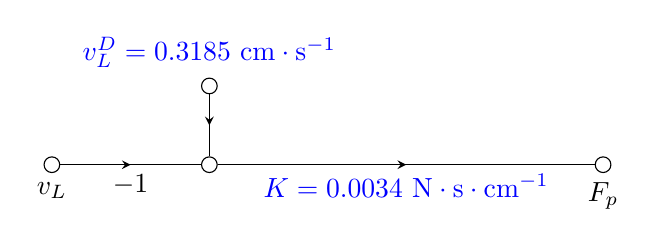
\begin{tikzpicture}
[
label revd/.is if=labrev,
%label revd/.default=true,
amark/.style={
            decoration={             
                        markings,   
                        mark=at position {0.5} with { 
                                    \arrow{stealth},
                                    \iflabrev \node[above] {#1};\else \node[below] {#1};\fi
                        }
            },
            postaction={decorate}
},
terminal/.style 2 args={draw,circle,inner sep=2pt,label={#1:#2}},
]

%Place the nodes
\node[terminal={below}{$v_L$}] (a) at (0,0) {};
\node[terminal={above}{$\color{blue} v_L^D=0.3185 ~\mathrm{cm\cdot s^{-1}}$}] (b) at (2cm,1) {};
\node[terminal={below left}{}] (c) at (2cm,0) {};
\node[terminal={below }{$F_p$}] (d) at (7cm,0) {};


=%Draw the connections
\draw[amark=$-1$] (a) to (c);
\draw[amark=$$] (b) to (c);

\draw[amark=${\color{blue}K= 0.0034~\mathrm{N\cdot s\cdot {cm}^{-1}}}$] (c) to (d);
\end{tikzpicture}
\end{document}